\documentclass{article}\usepackage[]{graphicx}\usepackage[]{color}
%% maxwidth is the original width if it is less than linewidth
%% otherwise use linewidth (to make sure the graphics do not exceed the margin)
\makeatletter
\def\maxwidth{ %
  \ifdim\Gin@nat@width>\linewidth
    \linewidth
  \else
    \Gin@nat@width
  \fi
}
\makeatother

\definecolor{fgcolor}{rgb}{0.345, 0.345, 0.345}
\newcommand{\hlnum}[1]{\textcolor[rgb]{0.686,0.059,0.569}{#1}}%
\newcommand{\hlstr}[1]{\textcolor[rgb]{0.192,0.494,0.8}{#1}}%
\newcommand{\hlcom}[1]{\textcolor[rgb]{0.678,0.584,0.686}{\textit{#1}}}%
\newcommand{\hlopt}[1]{\textcolor[rgb]{0,0,0}{#1}}%
\newcommand{\hlstd}[1]{\textcolor[rgb]{0.345,0.345,0.345}{#1}}%
\newcommand{\hlkwa}[1]{\textcolor[rgb]{0.161,0.373,0.58}{\textbf{#1}}}%
\newcommand{\hlkwb}[1]{\textcolor[rgb]{0.69,0.353,0.396}{#1}}%
\newcommand{\hlkwc}[1]{\textcolor[rgb]{0.333,0.667,0.333}{#1}}%
\newcommand{\hlkwd}[1]{\textcolor[rgb]{0.737,0.353,0.396}{\textbf{#1}}}%

\usepackage{framed}
\makeatletter
\newenvironment{kframe}{%
 \def\at@end@of@kframe{}%
 \ifinner\ifhmode%
  \def\at@end@of@kframe{\end{minipage}}%
  \begin{minipage}{\columnwidth}%
 \fi\fi%
 \def\FrameCommand##1{\hskip\@totalleftmargin \hskip-\fboxsep
 \colorbox{shadecolor}{##1}\hskip-\fboxsep
     % There is no \\@totalrightmargin, so:
     \hskip-\linewidth \hskip-\@totalleftmargin \hskip\columnwidth}%
 \MakeFramed {\advance\hsize-\width
   \@totalleftmargin\z@ \linewidth\hsize
   \@setminipage}}%
 {\par\unskip\endMakeFramed%
 \at@end@of@kframe}
\makeatother

\definecolor{shadecolor}{rgb}{.97, .97, .97}
\definecolor{messagecolor}{rgb}{0, 0, 0}
\definecolor{warningcolor}{rgb}{1, 0, 1}
\definecolor{errorcolor}{rgb}{1, 0, 0}
\newenvironment{knitrout}{}{} % an empty environment to be redefined in TeX

\usepackage{alltt}
\usepackage{amscd, amssymb, amsmath, verbatim, setspace}
\usepackage[left=1.0in, right=1.0in, top=1.0in, bottom=1.0in]{geometry}
\usepackage{mathrsfs}
\usepackage{listings}


\IfFileExists{upquote.sty}{\usepackage{upquote}}{}
\begin{document}
\begin{flushright}
  Arif Ali\\
  ANLY-511 Prob. Modeling \& Stat. Computing\\
	Nov 29, 2015\\
\end{flushright}

\begin{center}
  \LARGE\textbf{Homework \#10}
\end{center}
\section*{Exercise 73}
\begin{knitrout}
\definecolor{shadecolor}{rgb}{1, 1, 1}\color{fgcolor}\begin{kframe}
\begin{verbatim}
t_formula_confidence_interval = function(xhat, SD, ciLevel, sample_size){
  t_score = qt(1-((1-ciLevel)/2), sample_size-1)
  SE = SD/sqrt(sample_size) 
  return(c(xhat - t_score*SE, xhat + t_score*SE))
}
t_formula_confidence_interval(18.05, 5, .90, 20)
## [1] 16.11677 19.98323
\end{verbatim}
\end{kframe}
\end{knitrout}
I am 95\% confident that the population mean is between 16.11677 and 19.98323.
\section*{Exercise 74}
\begin{knitrout}
\definecolor{shadecolor}{rgb}{1, 1, 1}\color{fgcolor}\begin{kframe}
\begin{verbatim}
Spruce <- read.csv("~/Dropbox/School/Georgetown/Analytics 511 Fall 2015/ChiharaHesterberg/Spruce.csv")
boxplot(Spruce$Ht.change)
hist(Spruce$Ht.change, breaks = 20)
qqnorm(Spruce$Ht.change)
qqline(Spruce$Ht.change)
t_formula_confidence_interval(mean(Spruce$Ht.change), 
                              sd(Spruce$Ht.change), 
                              .95, length(Spruce$Ht.change))
## [1] 28.33685 33.52982
\end{verbatim}
\end{kframe}
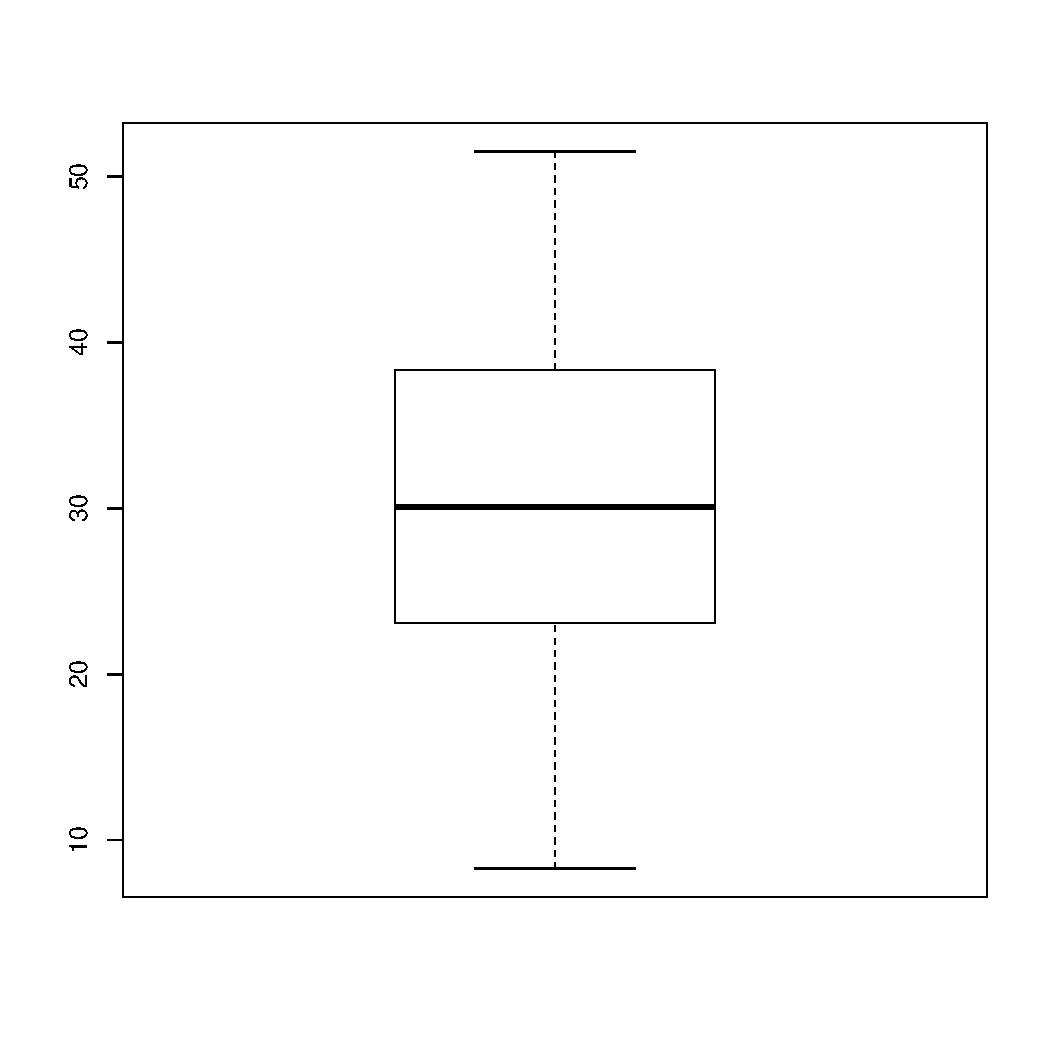
\includegraphics[width=0.33\linewidth]{figure/unnamed-chunk-3-1} 
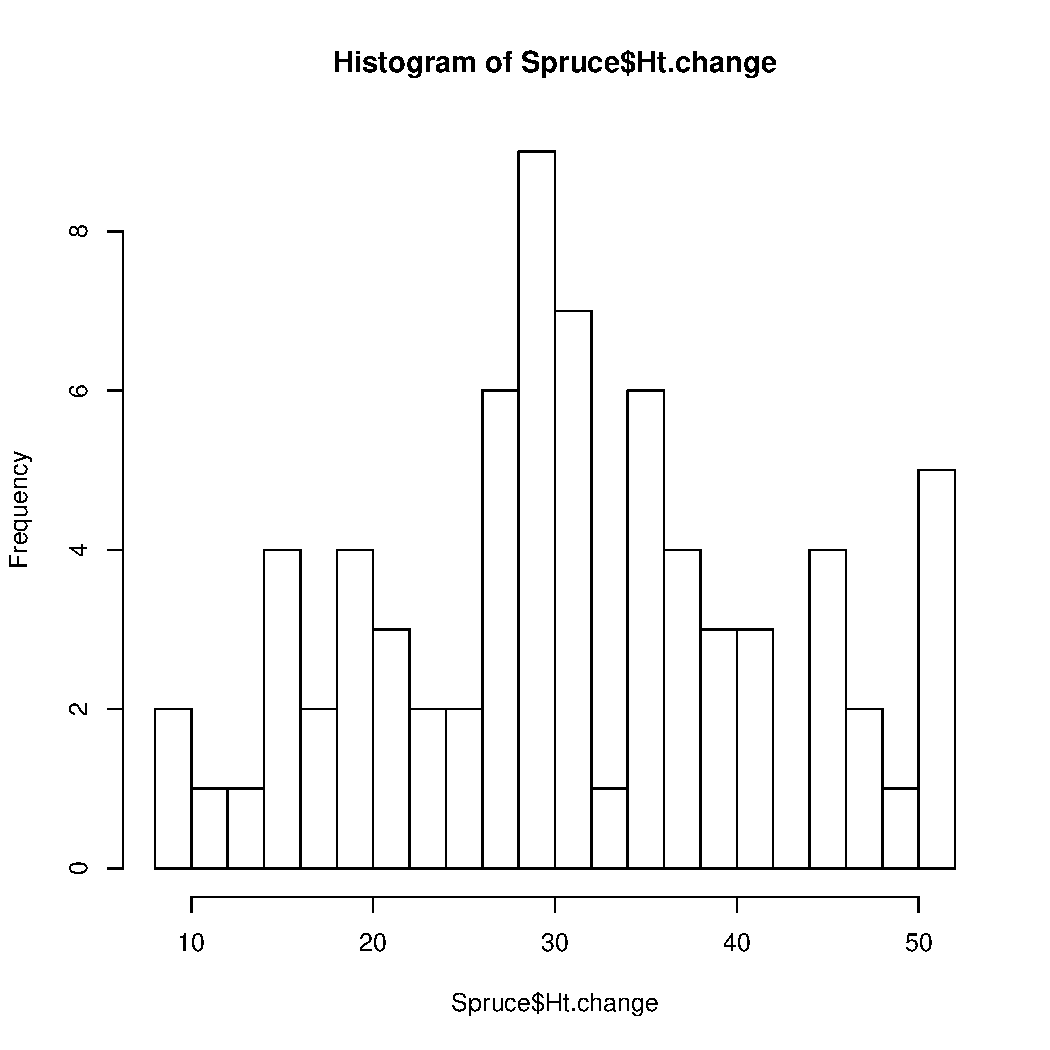
\includegraphics[width=0.33\linewidth]{figure/unnamed-chunk-3-2} 
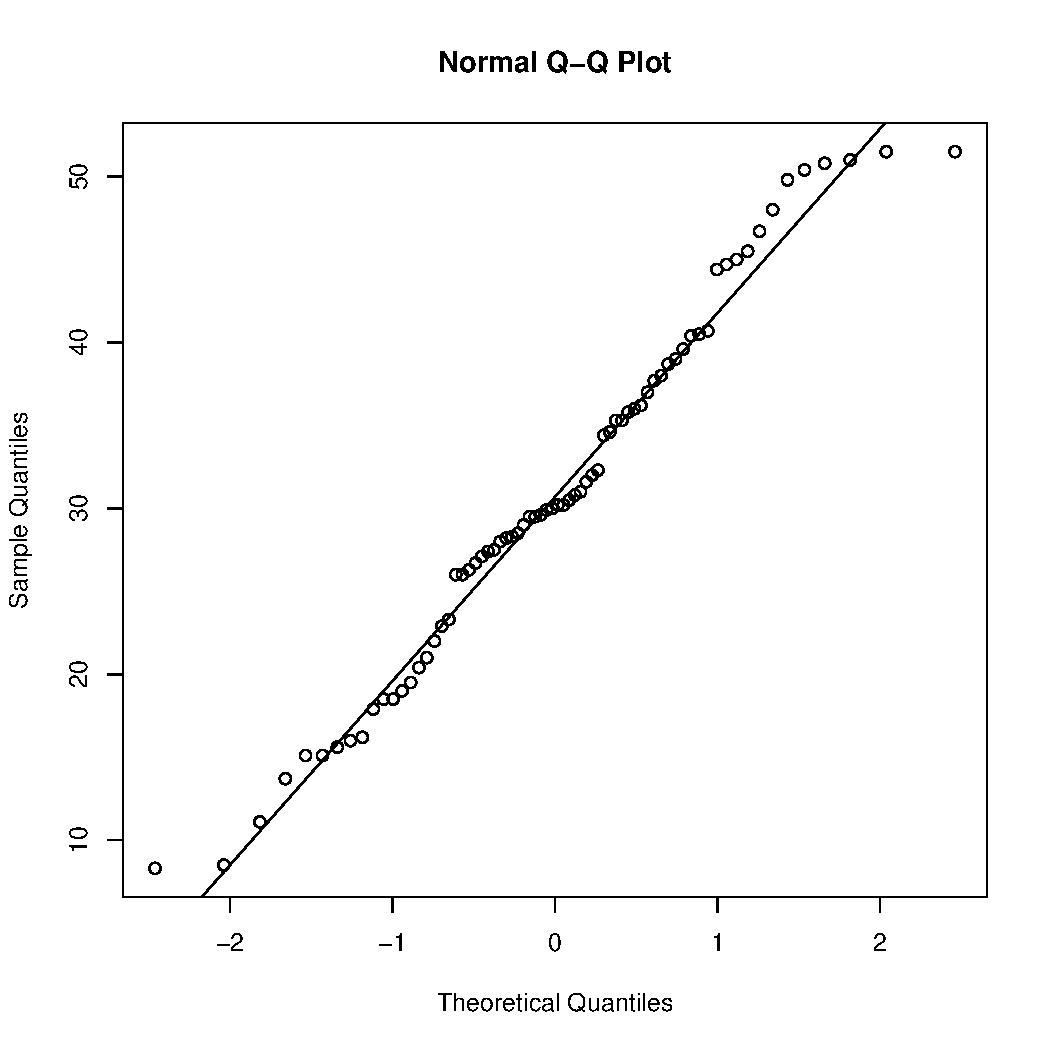
\includegraphics[width=0.33\linewidth]{figure/unnamed-chunk-3-3} 

\end{knitrout}
From the boxplot, it was interesting to see that the quantiles are spread out evenly (q2-q1=q4-q3=etc.). The histogram is very jumpy, so I can't say much about the distribution with respect to it. However, it takes on some resemblence of a bell curve. The qqnorm plot is interesting, because the data points "play" with the qqline. Thus, it seems to follow very close to a normal distribution. Based on the t-value Confidence Interval, there is a 95\% confidence that the population mean is between 28.33685 and 33.52982.


\section*{Exercise 75}
\begin{knitrout}
\definecolor{shadecolor}{rgb}{1, 1, 1}\color{fgcolor}\begin{kframe}
\begin{verbatim}
xhat = 5.8; yhat = 1.9 
sdx = 8.6; sdy = 4.2
sizex = 43; sizey = 36
sdxy = sqrt(sdx^2/sizex+sdy^2/sizey)
df = (sdx^2/sizex + sdy^2/sizey)^2/
  ((sdx^2/sizex)^2/(sizex-1)+(sdy^2/sizey)^2/(sizey-1))
t_score = qt(1-((1-.95)/2), df)
(xhat-yhat)+c(-t_score, t_score)*sdxy  
## [1] 0.9294237 6.8705763
\end{verbatim}
\end{kframe}
\end{knitrout}
Base on the interval, there is a 95\% confidence interval that the difference of the mean of weight loss between a low-carbohydrate diet and a ow-fat diet is between 0.9294237 and 6.8705763.
\section*{Exercise 76}
\subsection*{Part A}
\begin{knitrout}
\definecolor{shadecolor}{rgb}{1, 1, 1}\color{fgcolor}\begin{kframe}
\begin{verbatim}
Girls2004 <- read.csv("~/Dropbox/School/Georgetown/Analytics 511 Fall 2015/ChiharaHesterberg/Girls2004.csv")
boxplot(Girls2004$Weight~Girls2004$Smoker)

hist(Girls2004$Weight[Girls2004$Smoker=="No"], main = "Nonsmoker", breaks = 10)
hist(Girls2004$Weight[Girls2004$Smoker=="Yes"], main = "smoker", breaks = 10)
qqnorm(Girls2004$Weight[Girls2004$Smoker=="No"], main = "Nonsmoker")
qqline(Girls2004$Weight[Girls2004$Smoker=="No"])
qqnorm(Girls2004$Weight[Girls2004$Smoker=="Yes"], main = "smoker")
qqline(Girls2004$Weight[Girls2004$Smoker=="Yes"])
\end{verbatim}
\end{kframe}
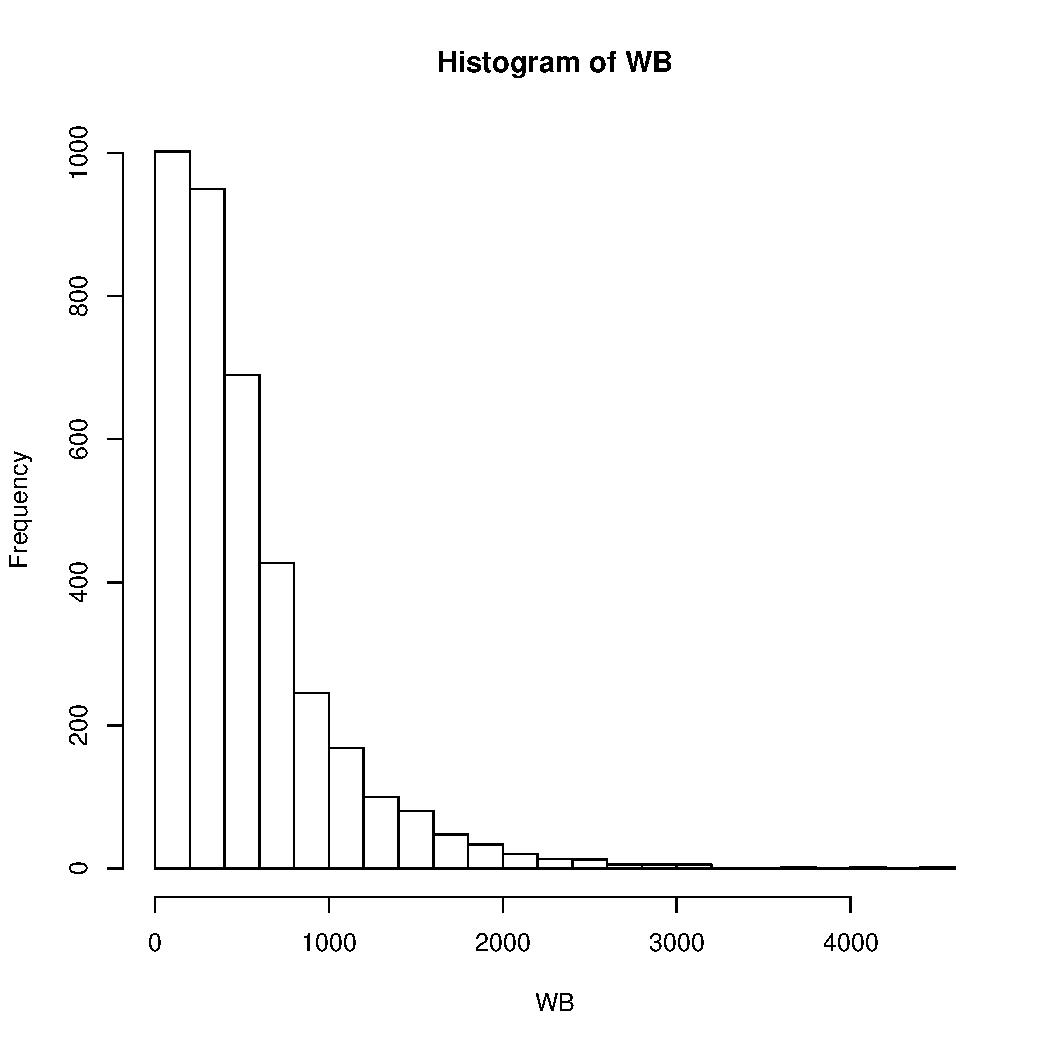
\includegraphics[width=0.33\linewidth]{figure/unnamed-chunk-5-1} 
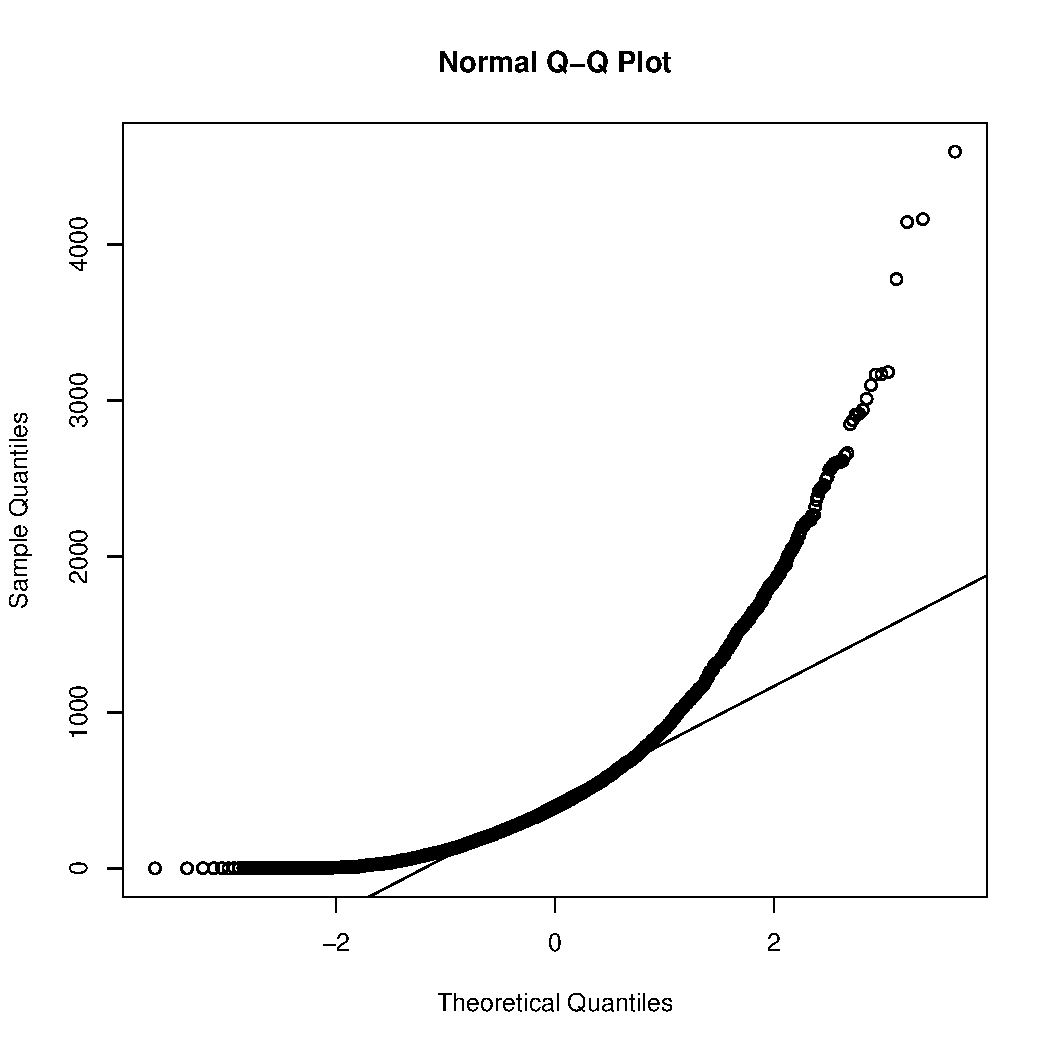
\includegraphics[width=0.33\linewidth]{figure/unnamed-chunk-5-2} 
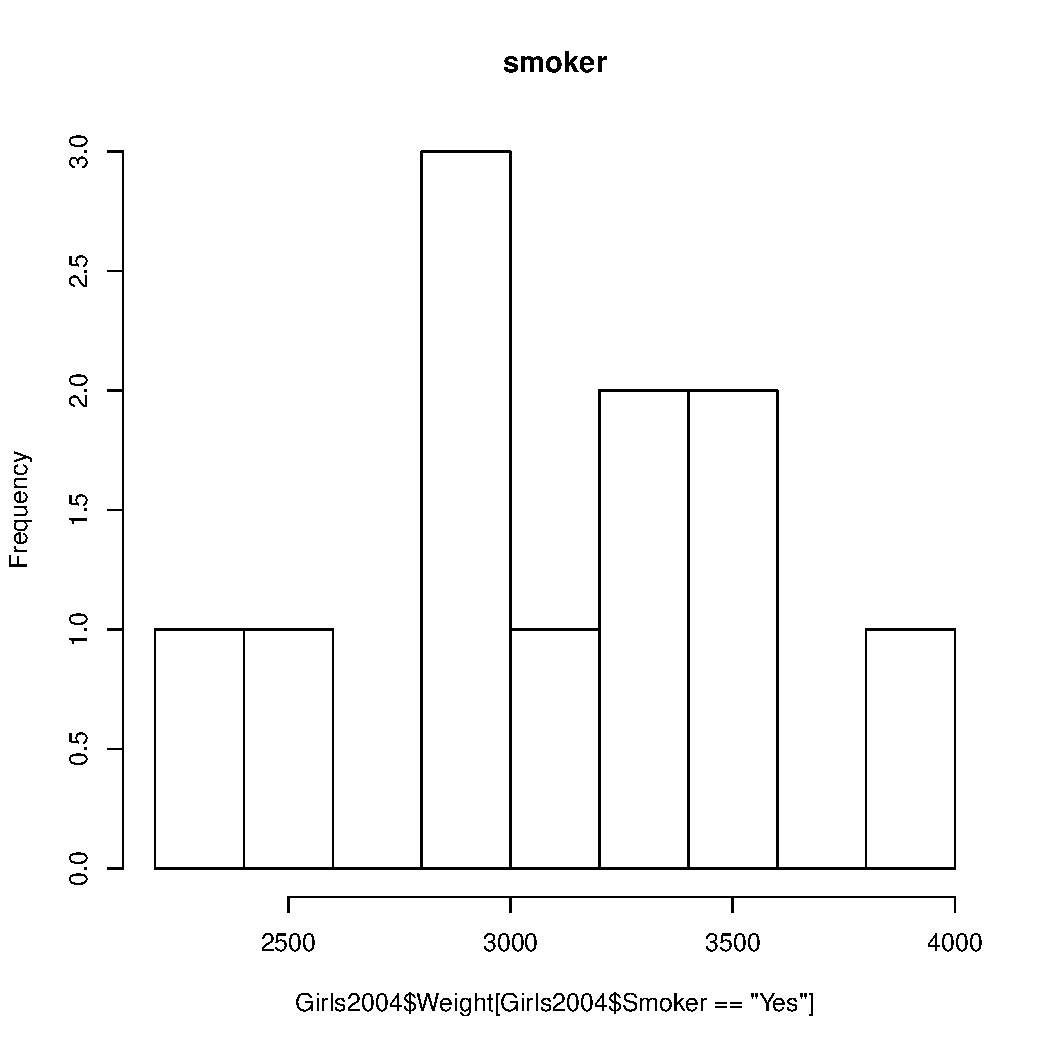
\includegraphics[width=0.33\linewidth]{figure/unnamed-chunk-5-3} 
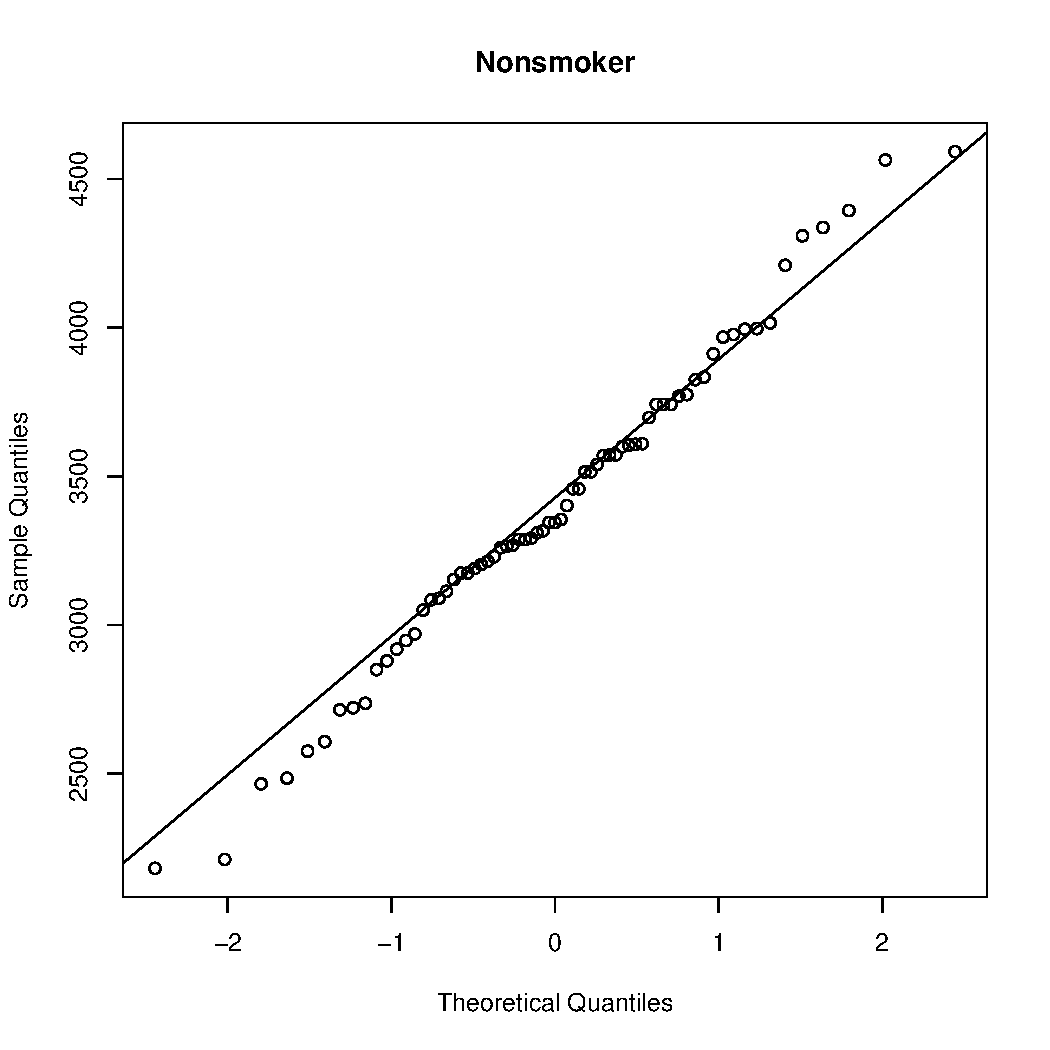
\includegraphics[width=0.33\linewidth]{figure/unnamed-chunk-5-4} 
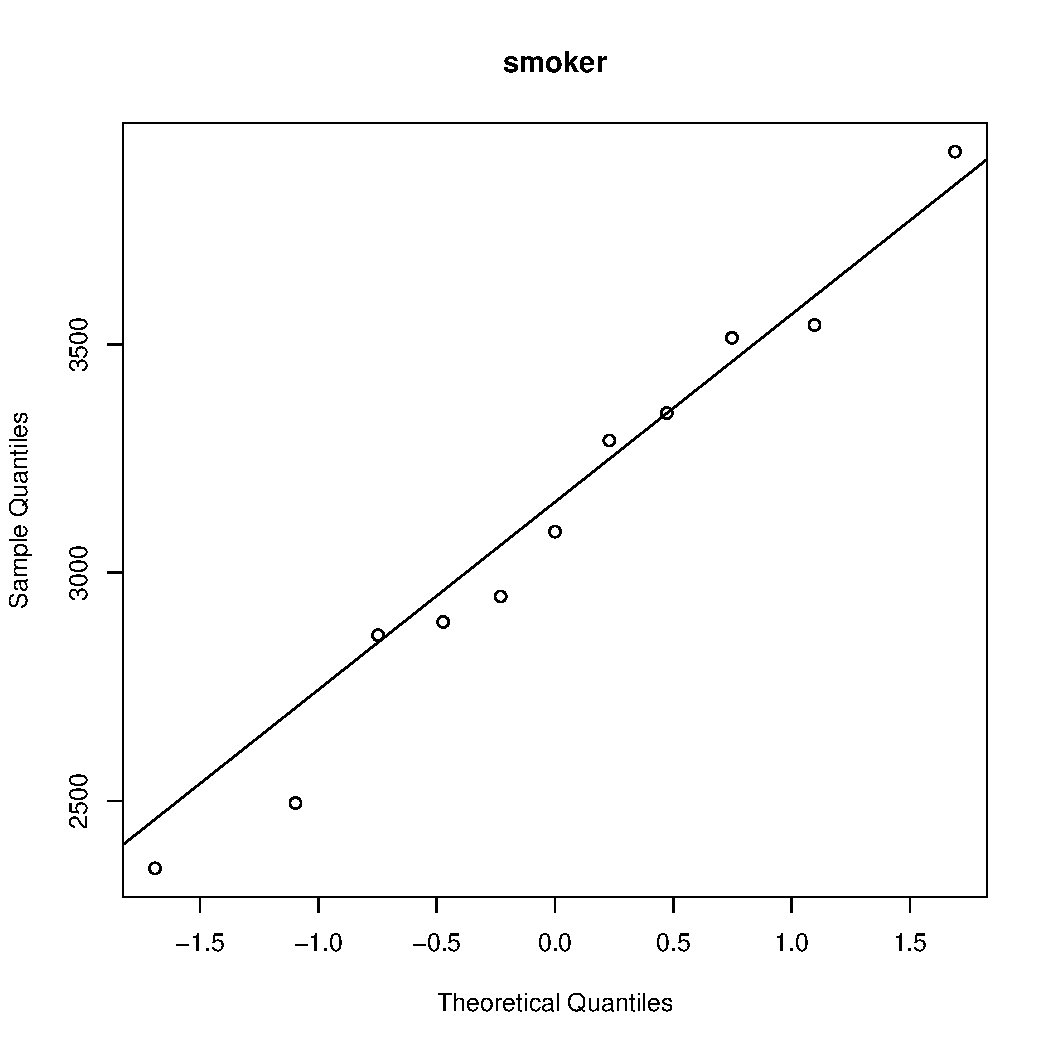
\includegraphics[width=0.33\linewidth]{figure/unnamed-chunk-5-5} 

\end{knitrout}
Based solely on the boxplot, it's clear that the distribution of the weight is higher for babies with non-smoking moms as opposed to smoking moms.
\subsection*{Part B}
\begin{knitrout}
\definecolor{shadecolor}{rgb}{1, 1, 1}\color{fgcolor}\begin{kframe}
\begin{verbatim}
xhat = mean(Girls2004$Weight[Girls2004$Smoker=="No"]) 
yhat = mean(Girls2004$Weight[Girls2004$Smoker=="Yes"])
sdx = sd(Girls2004$Weight[Girls2004$Smoker=="No"])
sdy = sd(Girls2004$Weight[Girls2004$Smoker=="Yes"])
sizex = length(Girls2004$Weight[Girls2004$Smoker=="No"]) 
sizey = length(Girls2004$Weight[Girls2004$Smoker=="Yes"])
sdxy = sqrt(sdx^2/sizex+sdy^2/sizey)
df = (sdx^2/sizex + sdy^2/sizey)^2/
  ((sdx^2/sizex)^2/(sizex-1)+(sdy^2/sizey)^2/(sizey-1))
t_score = qt(.95, df)
(xhat-yhat)-t_score*sdxy 
## [1] 14.99055
\end{verbatim}
\end{kframe}
\end{knitrout}
I am 95\% confident that the population mean difference between nonsmokers and smokers is at least 14.99055. Since zero is not the interval, the two confidence interval do not overlap. 
\section*{Exercise 77}
\subsection*{Part A}
\begin{knitrout}
\definecolor{shadecolor}{rgb}{1, 1, 1}\color{fgcolor}\begin{kframe}
\begin{verbatim}
prop.test(459, 980, correct = F)$conf.int
## [1] 0.4373100 0.4996717
## attr(,"conf.level")
## [1] 0.95
\end{verbatim}
\end{kframe}
\end{knitrout}
There is 95\% confidence that the mean of women that voted for Bush is between 0.4373100 and 0.4996717
\subsection*{Part B}
\begin{knitrout}
\definecolor{shadecolor}{rgb}{1, 1, 1}\color{fgcolor}\begin{kframe}
\begin{verbatim}
prop.test(426, 759, correct = F)$conf.int
## [1] 0.5257409 0.5961717
## attr(,"conf.level")
## [1] 0.95
\end{verbatim}
\end{kframe}
\end{knitrout}
There is 95\% confidence that the mean of men that voted for Bush is between 0.5257409 and 0.5961717
\subsection*{Part C}
\begin{knitrout}
\definecolor{shadecolor}{rgb}{1, 1, 1}\color{fgcolor}\begin{kframe}
\begin{verbatim}
prop.test(c(459,426), c(980,759), correct = F)$conf.int 
## [1] -0.14003926 -0.04575569
## attr(,"conf.level")
## [1] 0.95
\end{verbatim}
\end{kframe}
\end{knitrout}
There is a 95\% confidence that the difference of mean between the voting patterns of men and women is between -0.14003926 and -0.04575569 Since that interval does not include zero, there appears to be no overlap at the 95\% confidence level.
\section*{Exercise 78}
\subsection*{Part A}
In order for the two ranges to overlap, there must be a section of the range derived from both equations that "overlap". The best way to see that occurs is looking at the differences in the ranges which is $\hat{\theta_{1}}\pm 1.96*\hat{SE_{1}}-(\hat{\theta_{2}}\pm 1.96*\hat{SE_{2}})\implies\hat{\theta_{1}}-\hat{\theta_{2}}\pm 1.96*(\hat{SE_{1}}+\hat{SE_{2}})$.
Thus, in order to see that there is overlap, there must be 0 within the difference of the range as the corresponding over sections would zero out.

\subsection*{Part B}
$\hat{SE_{1}}+\hat{SE_{2}}>\sqrt{\hat{SE_{1}}^2+\hat{SE_{2}}^2}$ because $\hat{SE_{1}}\geq 0$ and $\hat{SE_{2}}\geq 0$.
$(\hat{SE_{1}}+\hat{SE_{2}})^2=\hat{SE_{1}}^2+2*\hat{SE_{1}}*\hat{SE_{2}}+\hat{SE_{2}}^2>\hat{SE_{1}}^2+\hat{SE_{2}}^2$

\subsection*{Part C}
The interval derived from Part A will be larger than that of Part B, since the bounds of part B are the square root of those from Part A. Since Part A will be a larger interval, it's probably going to be more likely that zero will be of the interval specified.


\section*{Exercise 79}
In order to figure out Exercise 79, I used www.milefoot.com/math/stat/ci-variances.htm to understand the idea behind the confidence interval for sample variance.

\begin{equation}
X_{1-\alpha/2}^{2}\leq\frac{(n-1)s^{2}}{\sigma^{2}}\leq X_{\alpha/2}^{2}\implies\frac{(n-1)s^{2}}{X_{\alpha/2}^{2}}\leq\sigma^{2}\leq\frac{(n-1)s^{2}}{X_{1-\alpha/2}^{2}}
\end{equation}


So the upper bound must be $\frac{(n-1)s^{2}}{X_{\alpha}^{2}}$.
\begin{knitrout}
\definecolor{shadecolor}{rgb}{1, 1, 1}\color{fgcolor}\begin{kframe}
\begin{verbatim}
sample79 = c(0.556, 7.267, 1.939, 1.907, 2.124, 1.334, 4.024, 0.455)

varcb = function(samp, ciLevel){
S = var(samp)
n = length(samp)
df = n-1
bound = qchisq(ciLevel, df)
ci = S*(df)/bound


return(ci)
}
varcb(sample79, .90)
## [1] 2.925507
\end{verbatim}
\end{kframe}
\end{knitrout}
We are 95\% confident that the variance is at most 2.925507, but not less than zero since variance must be greater than or eqaul to zero.
\section*{Exercise 80}
\subsection*{Part A}
\begin{knitrout}
\definecolor{shadecolor}{rgb}{1, 1, 1}\color{fgcolor}\begin{kframe}
\begin{verbatim}
Verizon <- read.csv("~/Dropbox/School/Georgetown/Analytics 511 Fall 2015/ChiharaHesterberg/Verizon.csv")
ILEC = Verizon[Verizon$Group=="ILEC","Time"]
hist(ILEC)
\end{verbatim}
\end{kframe}
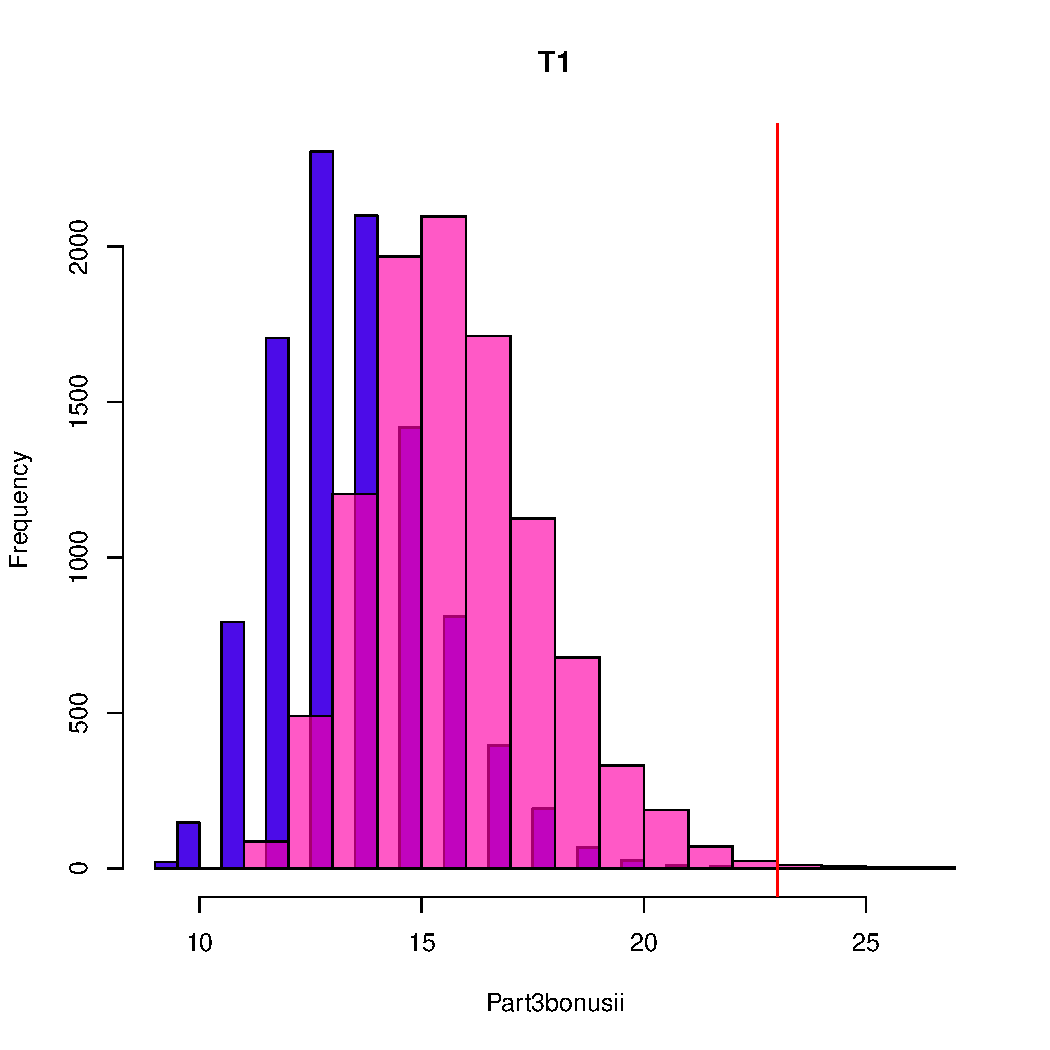
\includegraphics[width=0.33\linewidth]{figure/unnamed-chunk-11-1} 
\begin{kframe}\begin{verbatim}
alpha = .95
z <- replicate(10000,mean(sample(ILEC,size = length(ILEC), replace = T)))

# confidence interval

quantile(z,c((1-alpha)/2,(1+alpha)/2))
##     2.5%    97.5% 
## 7.725431 9.140905
t.test(ILEC)$conf.int
## [1] 7.705276 9.117945
## attr(,"conf.level")
## [1] 0.95
\end{verbatim}
\end{kframe}
\end{knitrout}
The difference between the two intervals is barely .02 for the lower bound of the interval and approximately 0.03 for the upper bound of the interval. However, the confidence interval from the the t test is slightly smaller, so I would use that confidence interval. There is a significant amount of overlap between the two. Based on the histogram, the looks like the data for ILEC is skewed. Based on the discussion board topic, the bootstrap method would be better
\subsection*{Part B}
\begin{knitrout}
\definecolor{shadecolor}{rgb}{1, 1, 1}\color{fgcolor}\begin{kframe}
\begin{verbatim}
CLEC = Verizon[Verizon$Group=="CLEC","Time"]
hist(CLEC)
\end{verbatim}
\end{kframe}
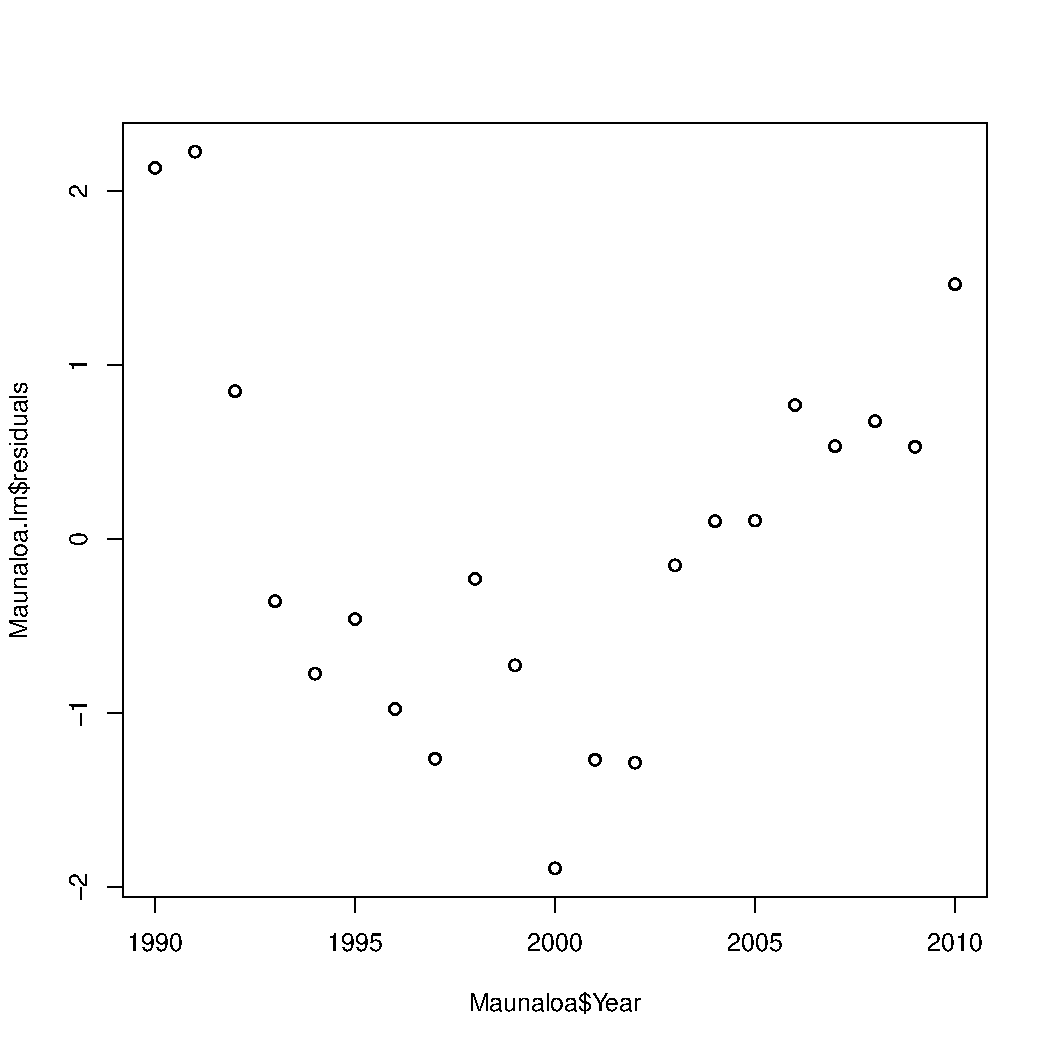
\includegraphics[width=0.33\linewidth]{figure/unnamed-chunk-12-1} 
\begin{kframe}\begin{verbatim}
alpha = .95
z <- replicate(10000,mean(sample(CLEC,size = length(CLEC), replace = T)))

# confidence interval

quantile(z,c((1-alpha)/2,(1+alpha)/2))
##     2.5%    97.5% 
## 10.17341 25.54421
t.test(CLEC)$conf.int
## [1]  8.075152 24.943109
## attr(,"conf.level")
## [1] 0.95
\end{verbatim}
\end{kframe}
\end{knitrout}
In terms of the lower bound, there is a drastic difference on the lower bound. This is probably because the sample size is extremely small. In this case, I would use the bootstrap quantile method because the interval is smaller. This concurs with the discussion board, which states "...that the t-test based CI loses accuracy for small samples and/or highly skewed distributions. "  
\end{document}
